\chapter{Implementation}

\paragraph*{}
The goal of the implementation is to guarantee that the executable memory pages that are loaded into the memory are not tampered with. In general, this is achieved through RA where the device proves its trustworthiness to a remote verifier, in this case, it is the trusted base of the device itself that checks the integrity of the REE. This integrity check is achieved by measuring the code pages of the processes in advance, for instance, during the installation of the particular code. This measurement can be done in a variety of ways. In this thesis, hashing was chosen because of its common use and it being well understood by the community. After these initial measurements have been taken, they need to be stored in a secure place. The secure memory of the PinePhone provided by ARM TrustZone was chosen because it can guarantee the integrity and confidentiality of the data. Last but not least, these measurements need to be retaken by a trusted base (SW) during execution time, and they need to be compared with the initial measurements to verify whether the running code has been tampered with. These runtime checks need to happen continuously to guarantee no modifications are introduced, or that the changes are observed before they can damage the system too much. Measuring code all the time is of course not feasible. Periodic measurements are more appropriate, but they should be scheduled unpredictably to avoid Time Of Check to Time Of User (TOC-TOU) attacks.

\section{NW application}

\paragraph*{}
The NW application (CA in figure \ref{implementation}) begins with looking up the processes that are currently running by examining the \textit{/proc} directory (1). This directory stores all relevant information concerning processes in Linux. In this directory there is a collection of directories named with numbers. These numbers represent the Process IDentifiers (PID). The PID is used within Linux to allow the operating system to differentiate between the different processes and manage them. It is of course necessary to attest all these processes. However, the explanation will focus on just one, for now, to keep things clear. Take for instance the directory \textit{/proc/1}, which will always exist since PID 1 is associated with \textit{proc\_init} which is the initial process the Linux OS forks. Within this directory there are two important files: \textit{pagemap} and \textit{maps}. The \textit{maps} file gives an overview of the different memory regions associated with the process. Besides the virtual address range, other information is also present, for instance, whether the pages are executable or writable, and where their symbolic origin is in the file structure. The \textit{pagemap} file, on the other hand, is necessary to translate from virtual address to physical address.

\begin{figure}[h]
\centering
\includegraphics[width=\textwidth]{implementation}
\caption{Process measurement sequence}
\label{implementation}
\end{figure}

\paragraph*{}
Translating the virtual addresses that are found in the \textit{proc/pid/maps} file into physical addresses, is based on a solution from \cite{cirosantilli}. The solution investigates the \textit{proc/pid/pagemap} file and generates a \textit{pagemap\_entry} from it. This \textit{pagemap\_entry} is used to structure the information associated with one entry in the \textit{maps} file. Based on this \textit{pagemap\_entry} the physical address can be derived from the virtual address found in the \textit{maps} file. Do note, that the \textit{maps} file provides a contiguous virtual memory region. It is not guaranteed that the physical memory will also be contiguous, so the first virtual address of every page is translated into a physical address. Also, the virtual addresses in the \textit{maps} file are virtual addresses in the Linux environment, as seen on the bottom left side of figure \ref{implementation}. Pages are 4 KB large, so lots of virtual addresses are translated into physical ones. After the physical addresses are obtained, they are put together into a list, and a memory reference of this list is sent to the SW for further investigation.

\section{Measurement PTA}

\paragraph*{}
The PTA could be called directly if it is configured correctly but to keep things simple here the communication goes through a normal TA (2). The measurement PTA receives a memory reference with inside the buffer all the physical memory addresses of the pages that need to be attested (3). Before the SW is able to access these memory pages, they need to be mapped into its virtual memory space (4). The mapping is done using the \textit{core\_mmu\_add\_mapping} function from the OP-TEE kernel \cite{OPTEEgit}. When this mapping is successful, the virtual address in the TEE (the right part of image \ref{implementation}) can be obtained using \textit{phys\_to\_virt}. The function \textit{phys\_to\_virt} returns the virtual address in the PTA where the memory can be accessed. With the PTA having access to the memory pages, the actual measurements can start. The hashing algorithm used is SHA-256, which can easily be substituted by another algorithm provided in the OP-TEE library. The hashing algorithms are provided by the OP-TEE framework and are easily usable from within the PTA.

\paragraph*{}
In the initialization phase of the integrity checking, the hash digests are stored in the secure memory of the device. The files written from the PTA to secure memory are only accessible by this PTA and are protected against everything in the NW. In this file, the hashes are sorted based on which \textit{pagemap\_entry} they come from and the page number within this region. Later, this allows to uniquely identify the hash value that will be used for comparison. After the initial hash values have been stored, the initialization phase is complete. This implies that the security of the stored measurement values is guaranteed, under the assumption that the SW does indeed protect the secure memory against access (read and write) from outside the SW. 

\paragraph*{}
During the attestation phase of the integrity checking, all the same steps will be taken as the initialization phase has taken up to this point, except for storing the calculated hash values. Instead, during this phase the newly calculated hash values will be compared with the hash values that are stored in the protected file where the initialization phase has written the measurement results. For the comparison, the hash value and the initial value are put into 4 \textit{uint64\_t} data types each. The first one from the hash is then compared with the first one of the initial value, the second one with the second one and so on, using the standard integer comparison functionality. The number of comparisons that fail is saved and printed in the debugging output stream of the SW. Ideally, the user should be notified about these faults, and which processes may experience an impact from this, based on whether the process uses the code for which the attestation has failed. Based on the information the user receives from the attestation, he can decide what action to take as the owner of the device.

\section{Improvements and extensions}

\paragraph*{}
First and foremost, it is very important to avoid relying on the rich OS for the translation of addresses, especially because this functionality is only possible with root privileges. This is because the data structures that contain this information are owned by the NW OS, and the necessary files are privileged which causes the accessibility issue. If possible this should be improved because an attacker in control of the rich OS could alter these data structures to hide the changed processes from the attestation PTA. The adversary could, for instance, keep an unchanged process hierarchy loaded in memory while the device is actually running on a different malicious process hierarchy. As long as it cannot be guaranteed that the addresses the SW receives are the addresses of the actual processes that are running, the attestation can be bypassed. 

\paragraph*{}
Secondly, the attestation currently only measures the executable pages present in RAM. The \textit{pagemap\_entry} only provides physical memory addresses for the pages that are loaded into RAM. This is sufficient during runtime, but for the initialization phase all the possible executable pages need to be measured to have a reference value to compare with. To achieve that, the entire code base of the process needs to be measured during the initialization phase. The binary files of the modules can be looked up to solve this issue. If it is possible to access these rich OS files from within the SW, they could also be attested as if they were loaded in memory. By measuring from these files, the initialization phase is not bound by the executable memory pages present in RAM anymore and can attest all pages. Having an initial value for all code pages is important to provide strong additional security guarantees. Measuring a memory page for the first time while the device is already deployed is bad practice, because there is no guarantee that the memory page has not been tampered with already. 

\paragraph*{}
A significant extension to allow this proof of concept to be turned into a complete attestation solution is to notify the user via trusted I/O. When informing the user about the results of the measurements, it is important to keep in mind the security of the channel on which this is achieved. ARM TrustZone provides trusted I/O paths which can be used for this goal. It could be used to inform the user of the problem, which program has been tampered with, or it could also take on a more coarse-grained approach like a Light Emitting Diode (LED) signal that some piece of software has failed the attestation, which is easier to achieve but less useful to the user. What details can be derived from this communication is not necessarily of the greatest importance. It is important how this communication works. To make sure the NW cannot interfere with the communication from the attestation PTA to the user, it should be implemented using the provided APIs of ARM Trusted Firmware-A (TFA) \cite{ARMfirmware}. Secure I/O paths are an extensively researched topic in the field of TEEs, for instance, to protect user data from compromised browsers \cite{EskandarianSaba2018FPUS} or to have a general trusted I/O path between the user and trusted services \cite{LiWenhao2014Btpo}. Using secure I/O is necessary to build a fully functional solution based on the proof of concept presented in this chapter. The secure I/O was not included in this work because no new functionality would be showcased and it would divert too much from the main focus of the implementation, namely checking the integrity of the NW processes.

\paragraph*{}
The second major extension focuses on the added security guarantees the attestation process provides. To achieve great security guarantees it is necessary to do more than just code attestation. Lots of software attacks are based on the used data structures and do not impact the text section of programs. As discussed in the background there are a variety of methods to detect software attacks based on used data structures and a great example of an extensive attestation method is \cite{MuhlbergJanTobias2016LaFT}. These forms of attestation are of course more complicated to execute and take a great amount of implementation effort. The attestation for this work was kept relatively simple to show that this form of attestation is achievable on the PinePhone. When designing a final product, it is of course encouraged to use more advanced techniques to increase the security guarantees of the code execution on the device.